Let $f(x)=x^2$ for $x\geq0$ and $f(x)=0$ for $x<0$.\\

a. Graph these functions.\\

b. Show $f$ is differentiable at $x=0$.\\

c. Calculate $f'$ on $\mathbb{R}$.\\

d. Is $f'$ continuous on $\mathbb{R}$? DIfferentiable on $\mathbb{R}$?\\\\

\begin{solution}\renewcommand{\qedsymbol}{}\ \\
    \begin{center}
        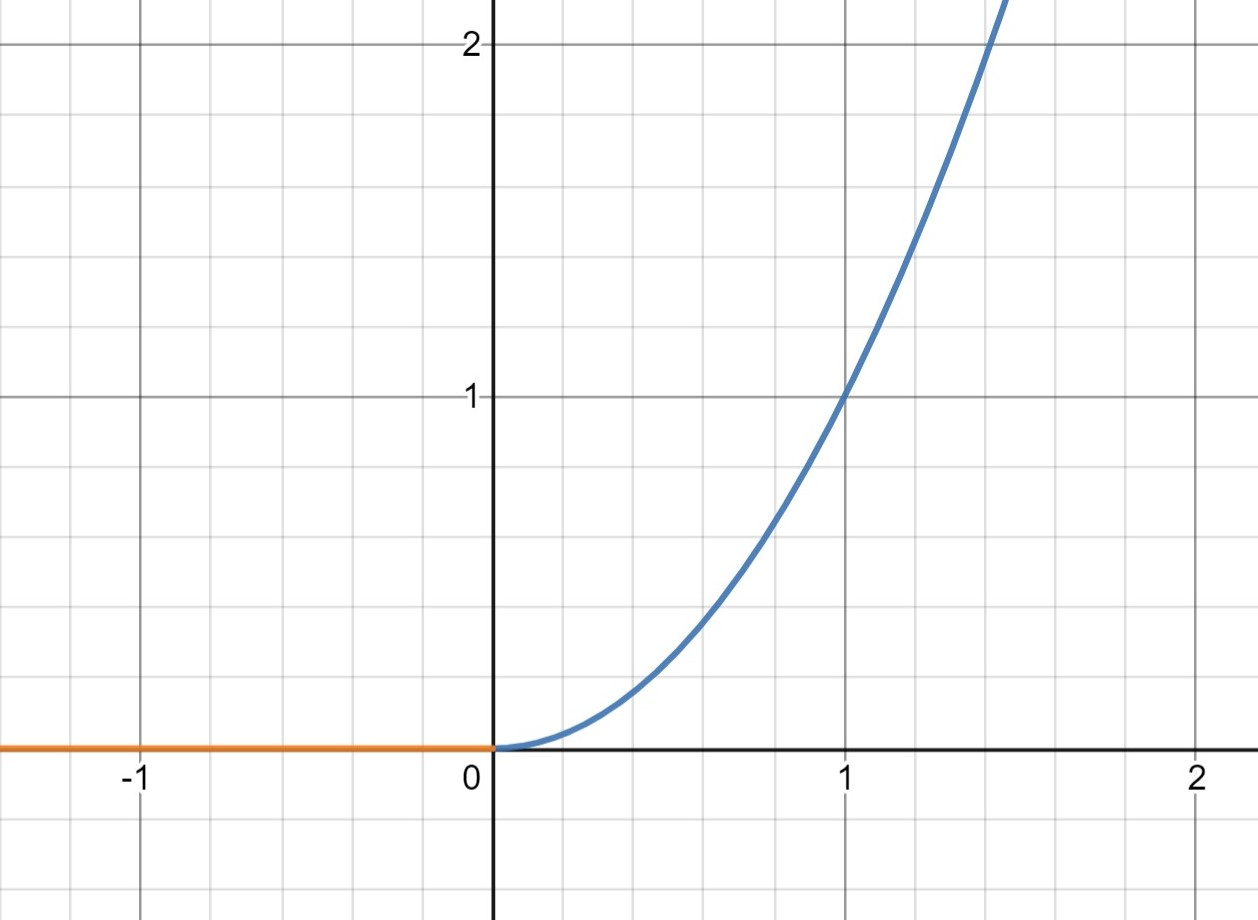
\includegraphics[scale=1]{graph.JPG}\\
    \end{center}

    Well, take $\frac{f(x)-f(0)}{x-0}$. Then
    
    $$\lim_{x\rightarrow0^-}\frac{f(x)-f(0)}{x-0}=\lim_{x\rightarrow0^-}\frac{0-0}{x-0}=0$$
    
    Also,
    
    $$\lim_{x\rightarrow0^+}\frac{f(x)-0}{x-0}=\lim_{x\rightarrow0^+}\frac{x^2}{x}$$
    $$=\lim_{x\rightarrow0^+}x=0$$
    
    Since the limit exists, is the same from both directions, and is finite, we get that $f$ is
    differentiable at $x=0$. In particular $f'(0)=0$\\

    Well $\frac{d}{dx}x^2=2x$ and $\frac{d}{dx}0=0$, so $f'(x)=2x$ for $x\geq0$ and $f'(x)=0$ for
    $x<0$.\\

    Well take any sequence $s_n$ such that $\lim_{n\rightarrow\infty}s_n=0$ where $s_n\neq0$ for all
    $n$. Then
    
    $$\lim_{n\rightarrow\infty}f(s_n)=\lim_{n\rightarrow\infty}2s_n$$
    $$=2\lim_{n\rightarrow\infty}s_n=2*0=0=f(0)$$
    
    Thus, $f'$ is continuous at $x=0$ and by continuity of ploynomials, is continuous everywhere else.
    $f$ is not differentiable on $\mathbb{R}$ as
    
    $$\lim_{x\rightarrow0^-}\frac{f(x)-f(0)}{x-0}=0\neq1=\lim_{x\rightarrow0^+}\frac{f(x)-f(0)}{x-0}$$

\end{solution}